\vspace{-4pt}

\section{Evaluation}
\label{sec:eval}

\begin{figure*}[t]
\captionsetup[subfigure]{labelformat=simple}
    \renewcommand\thesubfigure{(\alph{subfigure})}
\centering
\begin{subfigure}{0.32\textwidth}
    \centering
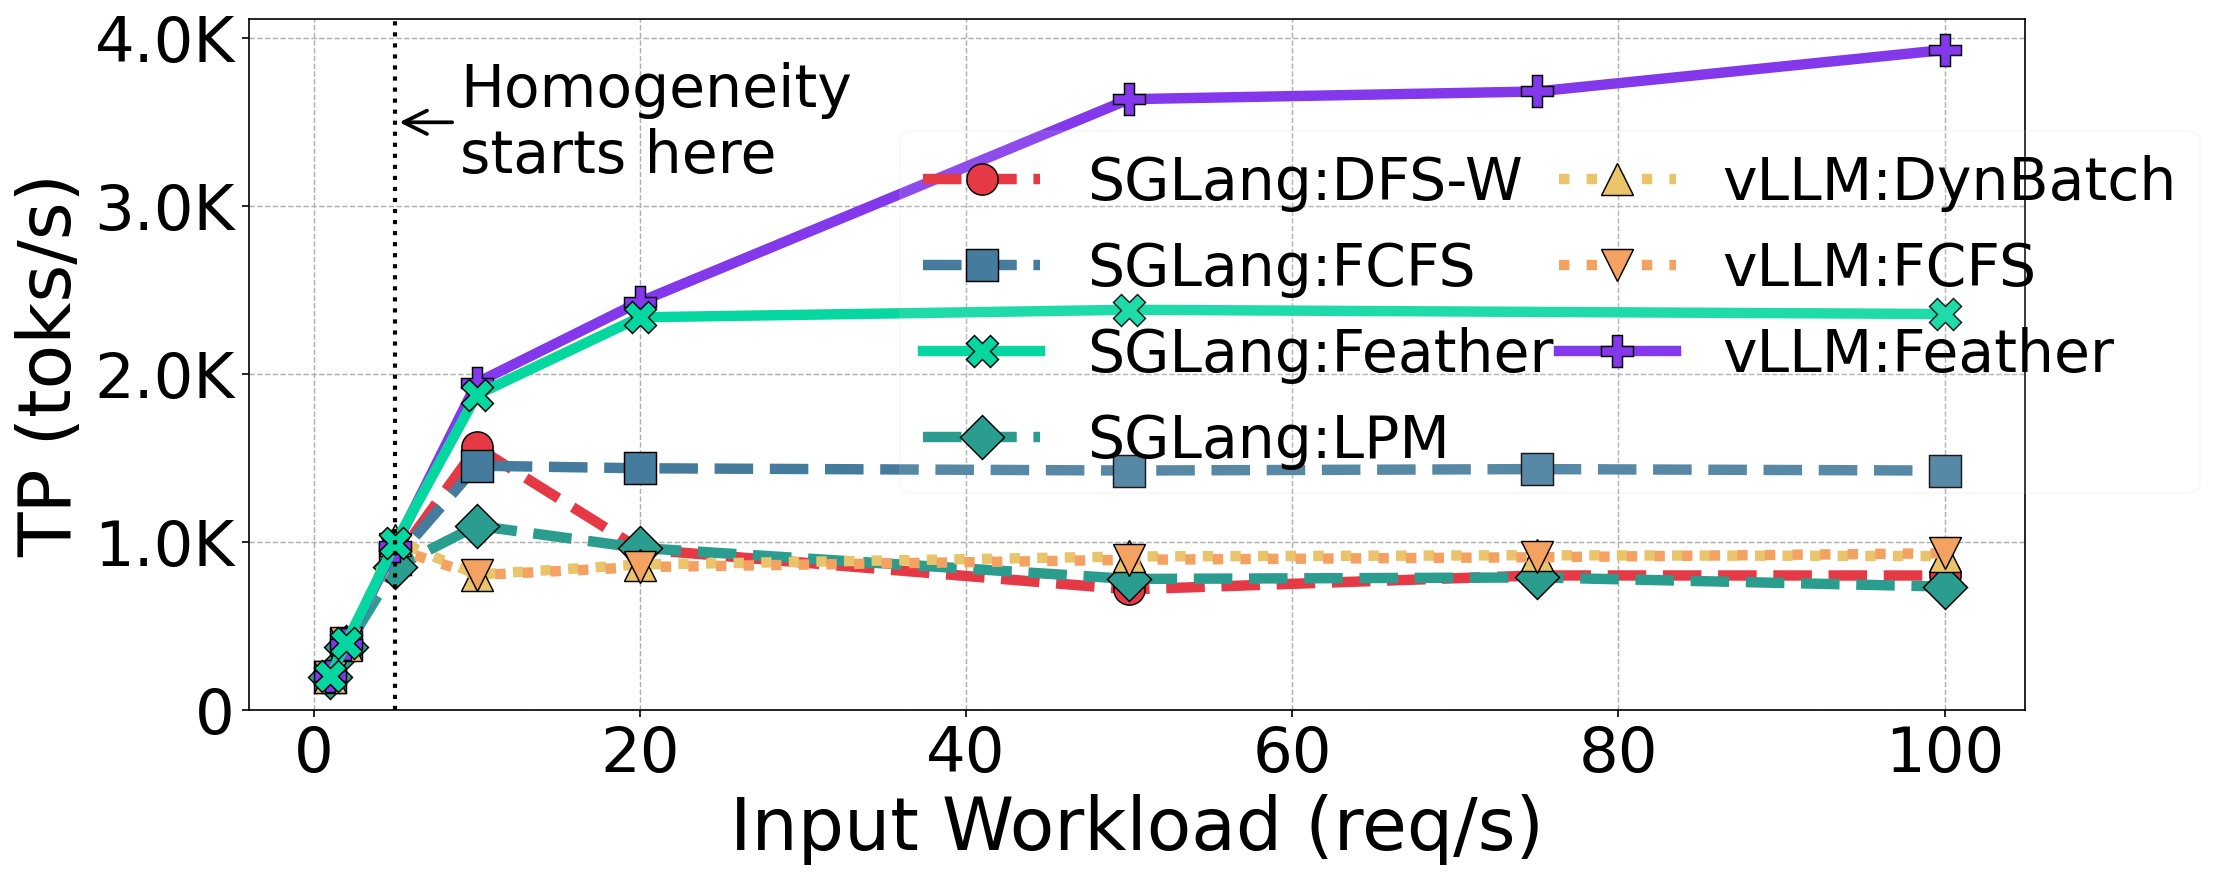
\includegraphics[width=\linewidth]{results/req_per_sec_plots/throughput_vs_rps.png}
\caption{Throughput}
\label{fig:tp_vs_rps_l_5000_fam_5}
\end{subfigure}
\hfill
\begin{subfigure}{0.32\textwidth}
    \centering
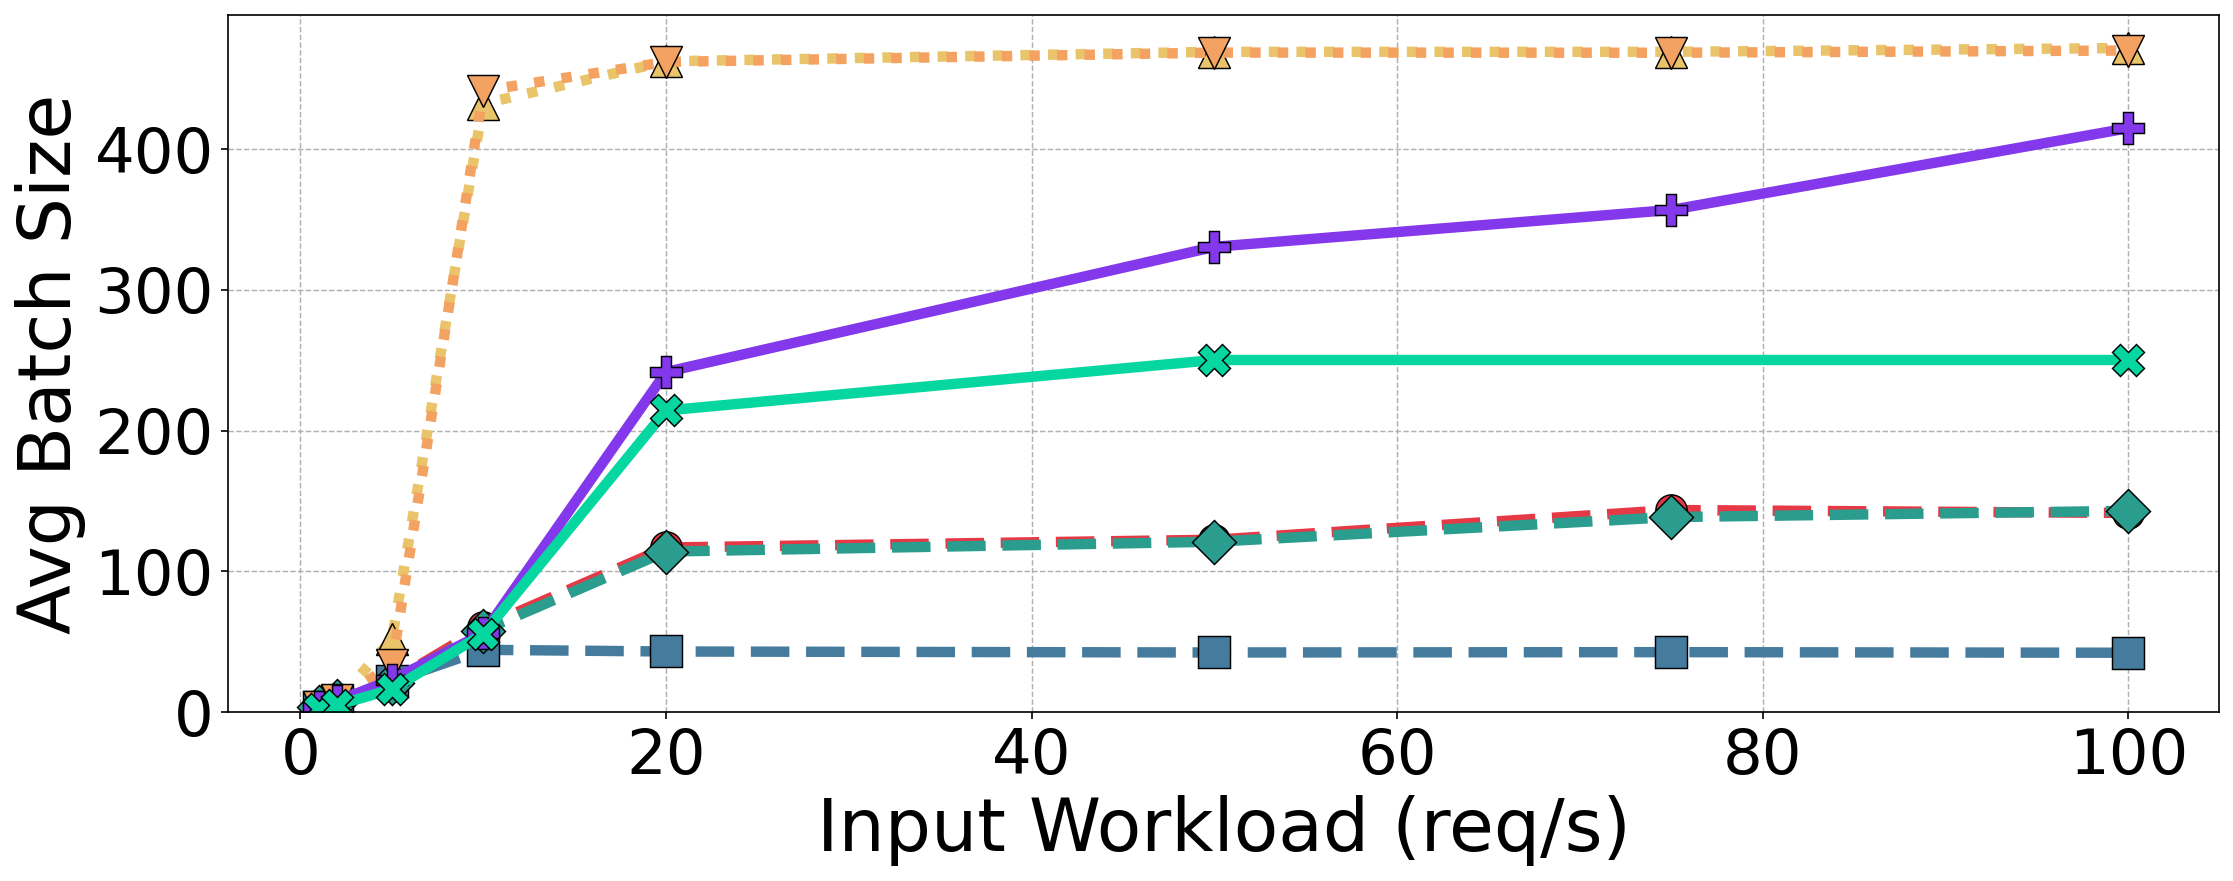
\includegraphics[width=\linewidth]{results/req_per_sec_plots/avg_batch_vs_rps.png}
\caption{Average Batch Size}
\label{fig:abs_vs_rps_l_5000_fam_5}
\end{subfigure}
\hfill
\begin{subfigure}{0.32\textwidth}
    \centering
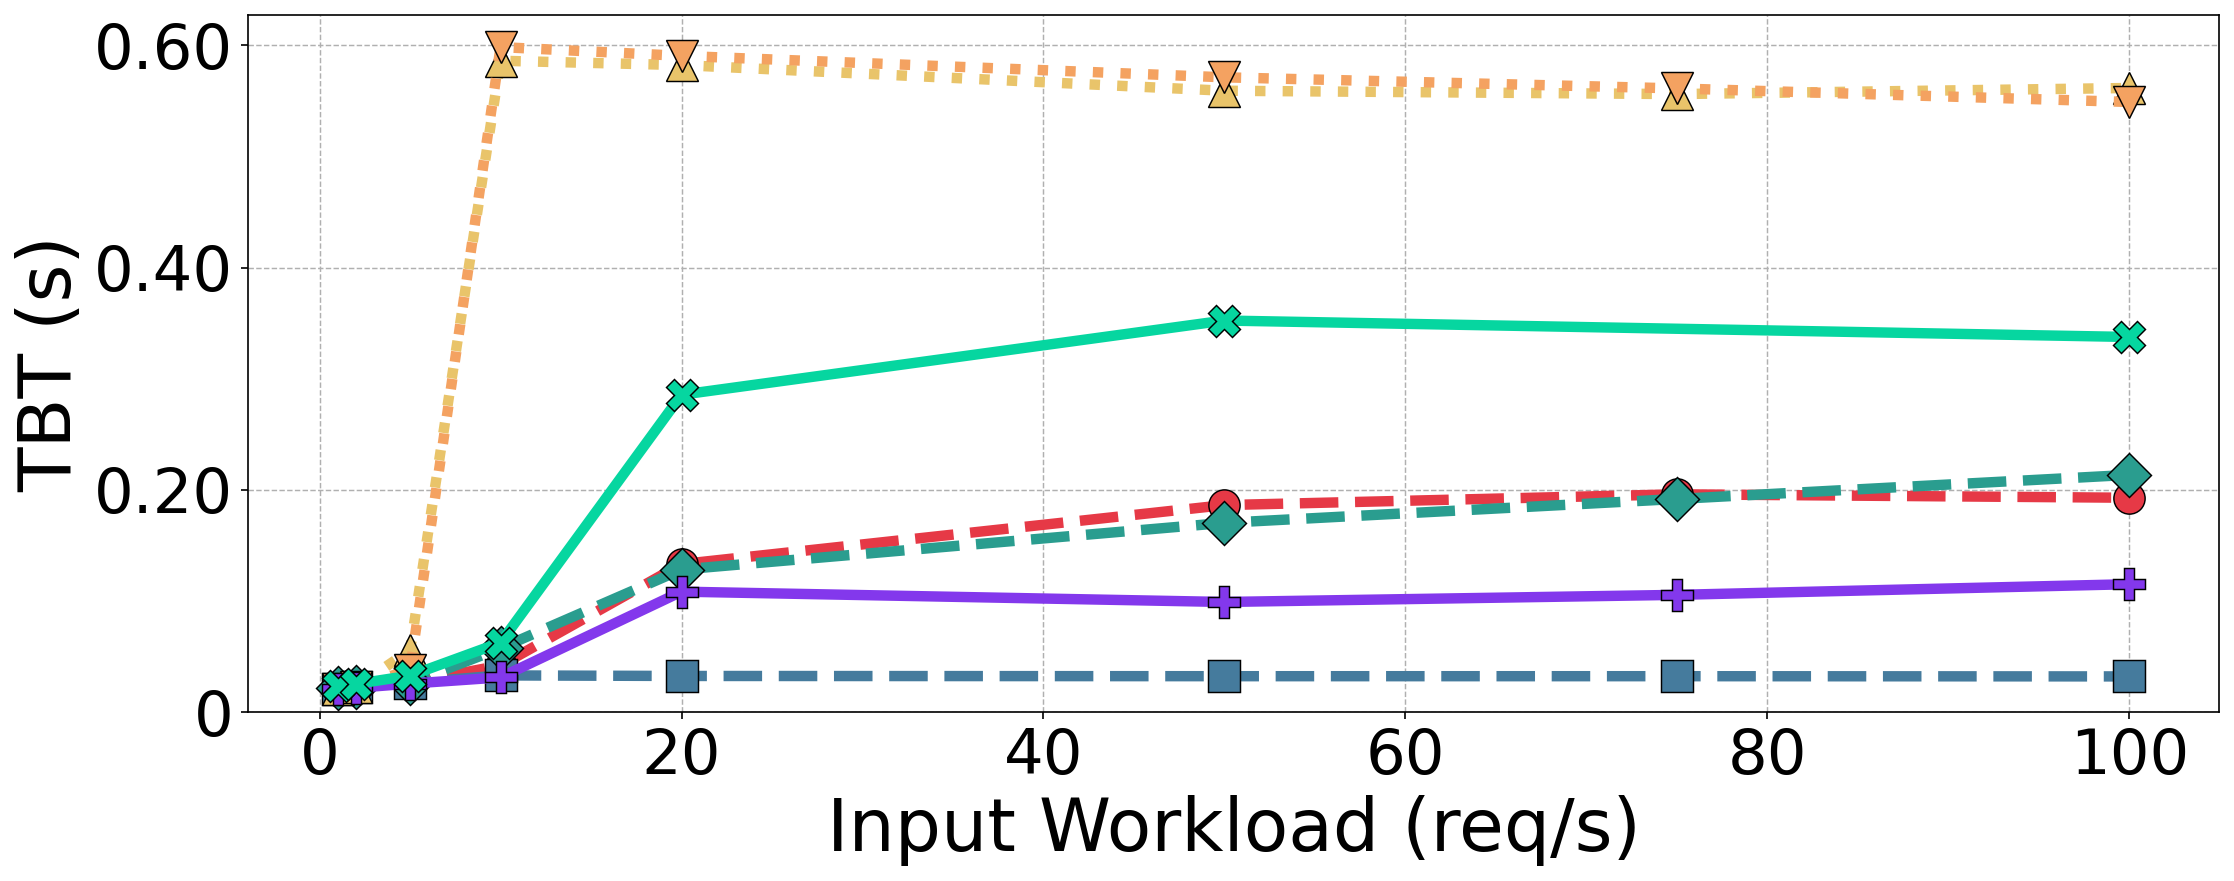
\includegraphics[width=\linewidth]{results/req_per_sec_plots/avg_timediff_vs_rps.png}
\caption{Time between tokens (TBT)}
\label{fig:tbt_vs_rps_l_5000_fam_5}
\end{subfigure}
\caption{Poisson Workload}
\label{fig:input_workload_poisson_rates}
\vspace{-13pt}
\end{figure*}

We evaluate \Feather across diverse models, GPU configurations, and real-world datasets and scenarios. Our evaluation answers the following questions: (i) Under what workloads do smaller homogeneous batches outperform larger heterogeneous ones? (ii) How effective is \Feather's Chunked Hash Tree compared to traditional radix-tree-based approaches? (iii) How do different design components of \Feather (RL, CHT) interact to produce end-to-end performance gains? 

\vspace{-4pt}

\subsection{Experimental Setup}
\subsubsection*{Models and Hardware}
We evaluate three model families across multiple sizes: Qwen 0.5B, 1.5B, 8B~\cite{qwen}, LLaMA 3 8B~\cite{llama3modelcard}, and LongChat 13B~\cite{longchat2023}. Experiments are run on an NVIDIA RTX 6000 Ada GPU~\cite{nvidia_rtx6000_datasheet} with 48 GB GDDR6, 96 MB L2, and the maximum batch size is fixed at 500, which fits within the GPU memory for most settings. We additionally evaluate on an A100-80GB GPU for comparisons involving PAT~\cite{yi2026pat}, as it is specifically optimized for this hardware.

\begin{figure}[t]
\captionsetup[subfigure]{labelformat=simple}
    \renewcommand\thesubfigure{(\alph{subfigure})}
\centering
\begin{subfigure}{0.49\columnwidth}
    \centering
    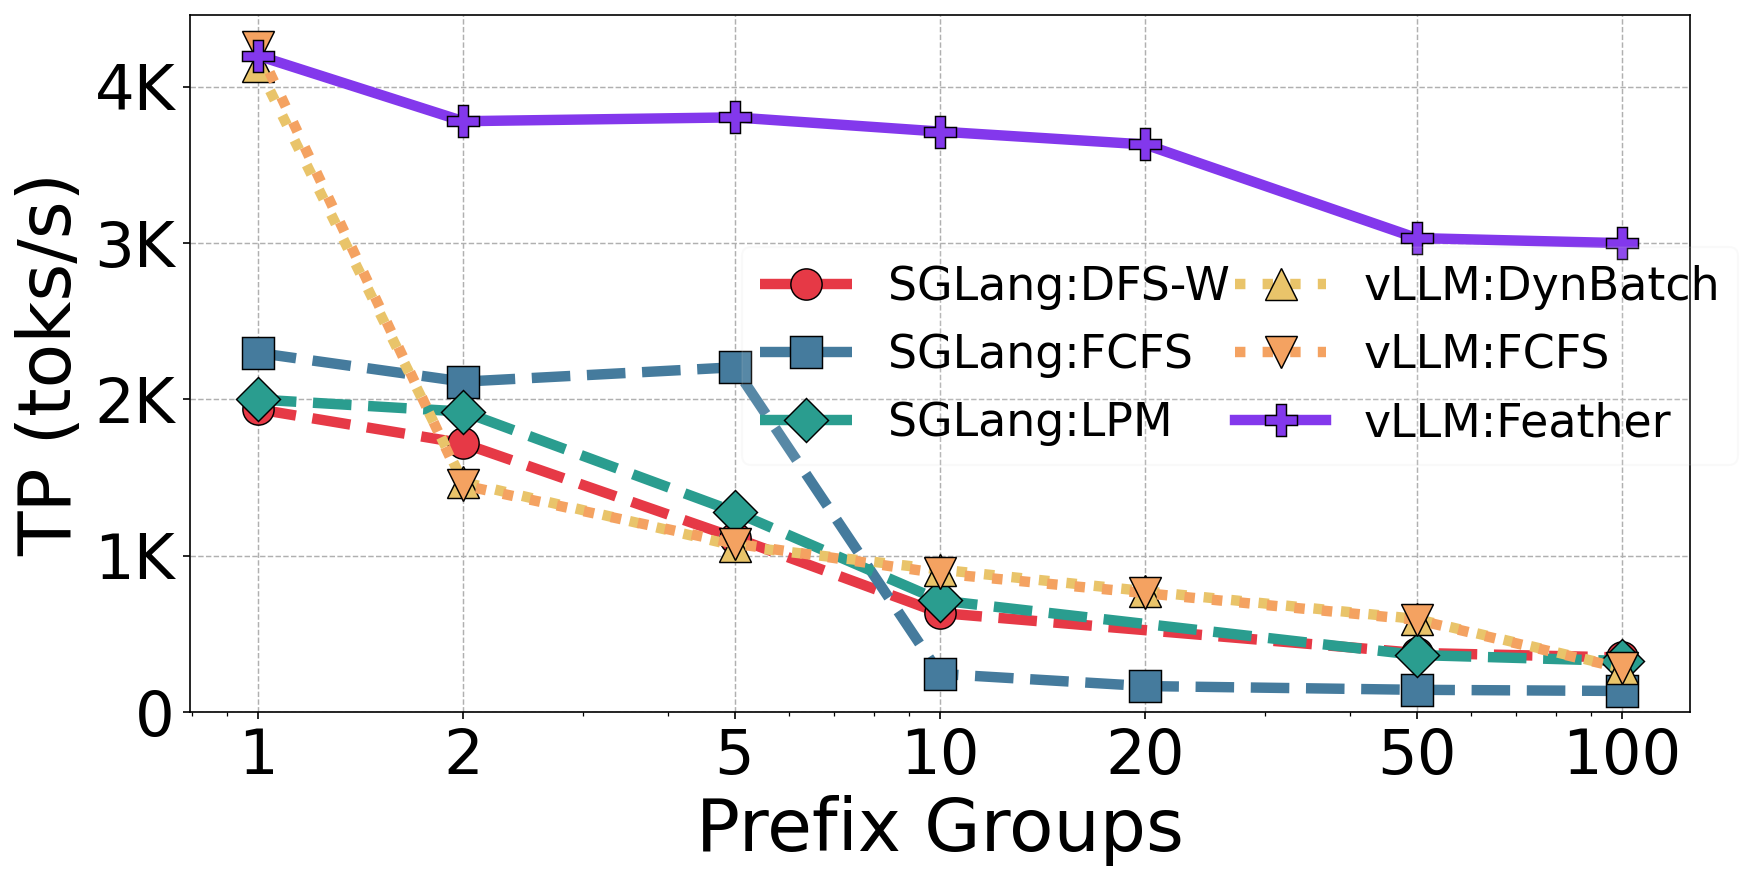
\includegraphics[width=\linewidth]{results/families_plots/throughput_vs_fam.png}
    \caption{Throughput}
    \label{fig:tp_vs_fam_l_5000}
\end{subfigure}
\hfill
\begin{subfigure}{0.49\columnwidth}
    \centering
    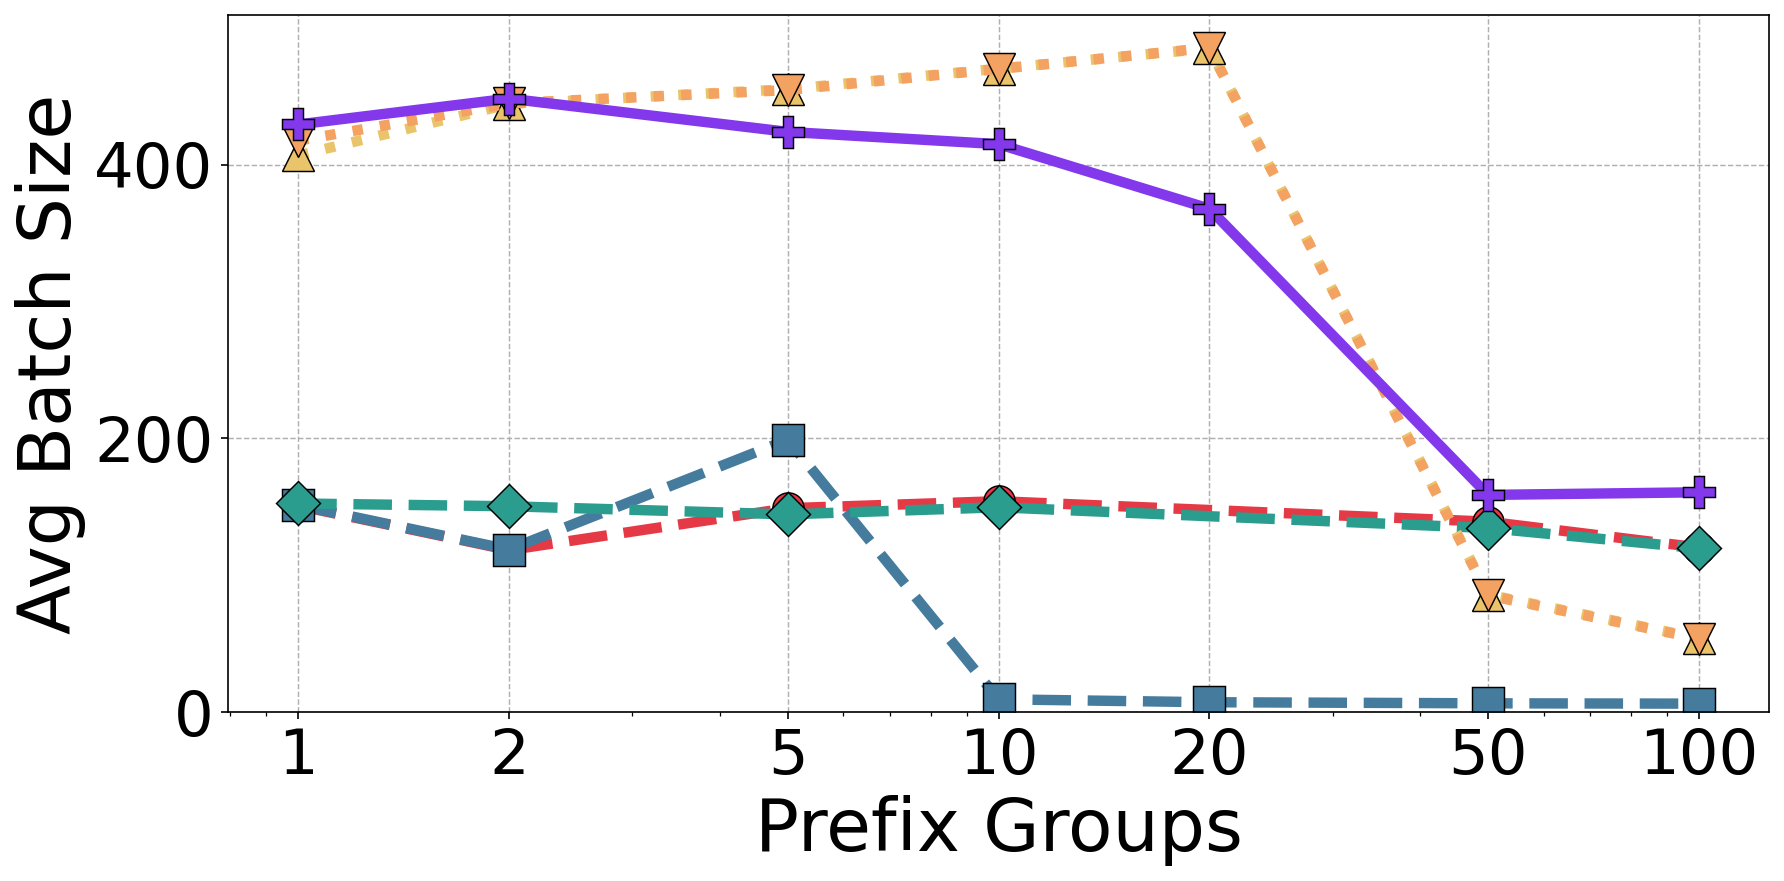
\includegraphics[width=\linewidth]{results/families_plots/avg_batch_vs_fam.png}
    \caption{Average Batch Size}
    \label{fig:abs_vs_fam_l_5000}
\end{subfigure}
\caption{Varying Number of Prefix Groups}
\label{fig:num_prefix_groups}
\vspace{-18pt}
\end{figure}

\vspace{-5pt}

\subsubsection*{Workloads}
Following prior work, request arrivals are modeled as a Poisson process, with length pruning applied as required by each experiment. L-Eval~\cite{an2023leval} is a benchmark of human-labeled query–response pairs spanning tasks such as summarization and question answering, with sequence lengths ranging from 2.7K to 210.5K tokens. LongBench~\cite{bai2024longbench2} is a collection of long-context samples across six task categories: multi-document QA, summarization, and code completion, with context lengths between 4K and 10K tokens.

\vspace{-5pt}

\subsubsection*{Baselines}
We compare \Feather against state-of-the-art LLM serving systems, all with prefix caching enabled. vLLM \cite{kwon2023efficient} uses its default FCFS scheduling policy. SGLang~\cite{zheng2024sglangefficientexecutionstructured} is evaluated under FCFS, LPM, and DFS-W to cover its design space. We also evaluate DynamicBatching~\cite{pang2025optimizing} and PAT~\cite{yi2026pat}, both implemented on top of vLLM: DynamicBatching adjusts batch sizes based on runtime memory utilization and latency constraints, while PAT is a prefix-aware attention kernel that reduces redundant KV cache accesses via query packing.

\vspace{-5pt}

\subsubsection*{Metrics}
We report three key metrics. Throughput (toks/s) measures the output tokens generated per second, reflecting serving capacity and GPU utilization. Time between tokens (TBT) measures the average interval between decoded tokens, reflecting responsiveness, especially in interactive settings. We also track the average batch size per forward pass to relate scheduling decisions to these metrics.

\vspace{-4pt}

\subsection{End-to-End Comparison: \Feather vs Baselines}
We evaluate a workload where the default configuration has 5 prefix groups\footnote{We also evaluate workloads without prefix sharing and show \Feather performs on par with FCFS (\S\ref{subsec:workloads_with_no_prefix_sharing}).}, each 5K tokens long, with roughly equal request distribution, a request rate of 100 req/s, and 200 output tokens per request. Such workload configurations are common in prior work~\cite{yi2026pat,MLSYS2025_96894468} evaluating LLM serving systems. We vary these parameters to examine how \Feather compares to the baselines. The token budget is 32K tokens. For \Feather's RL policy, we find that bandit and Q-learning approaches perform similarly across most settings; unless stated otherwise, we report results using the bandit policy. 

\vspace{-5pt}

\subsubsection*{Varying Input Request Rate}
Figure~\ref{fig:tp_vs_rps_l_5000_fam_5} shows throughput (toks/s) as a function of the request rate. Across all policies, throughput increases with the request rate before saturating. \Feather (on vLLM) consistently outperforms all baselines at every request rate. At 100 req/s, \Feather achieves roughly $4\times$ the throughput of vLLM (FCFS). Notably, this advantage is not driven by larger batch sizes. As shown in Figure~\ref{fig:abs_vs_rps_l_5000_fam_5}, \Feather in general maintains a \textit{smaller} average batch size than vLLM (FCFS), and beyond the vertical line shown in the plot, \Feather's RL policy decides to have completely homogeneous batches. This reinforces a key insight: \textit{smaller, homogeneous batches outperform larger, heterogeneous ones}. The gradual growth in \Feather's batch size with increasing request rate reflects its ability to efficiently aggregate more requests from the same prefix group into the active batch without sacrificing locality. SGLang policies consistently operate at smaller batch sizes than vLLM, as vLLM avoids double-counting shared prefix tokens toward the token budget, allowing more requests per batch. Dynamic Batching performs similarly to vLLM (FCFS), as all KV caches fit within GPU memory. Figure~\ref{fig:tbt_vs_rps_l_5000_fam_5} shows time between tokens (TBT). \Feather (on vLLM) achieves substantially lower TBT than all baselines except SGLang (FCFS), whose smaller batch sizes yield faster per-token generation. While SGLang's LPM and DFS-W policies also use small batch sizes, their TBT remains significantly higher than \Feather due to non-trivial scheduling overhead during batch construction.  \Feather implemented on SGLang also shows similar qualitative trends and outperforms all other SGLang policies. Unless otherwise stated, all subsequent results refer to \Feather implemented on vLLM.

\vspace{-5pt}

\subsubsection*{Varying Number of Prefix Groups}
Figures~\ref{fig:tp_vs_fam_l_5000} and \ref{fig:abs_vs_fam_l_5000} show throughput and average batch size as functions of the number of prefix groups. Increasing the number of prefix groups introduces greater request heterogeneity, reducing KV cache locality. This leads to a sharp throughput drop for vLLM (FCFS), even when increasing from 1 to 2 prefix groups. As the number of groups increases further, FCFS degrades rapidly: beyond 20 groups, the KV cache footprint exceeds HBM capacity, causing a sharp reduction in batch size and increased recomputation. \Feather mitigates this by grouping requests with shared prefixes, increasing KV cache reuse and avoiding premature evictions. As a result, \Feather maintains a more stable batch size and throughput across all prefix group configurations, significantly outperforming all baselines. At 100 prefix groups, \Feather achieves $10\times$ higher throughput than vLLM (FCFS). SGLang's LPM and DFS-W policies partially mitigate evictions, achieving higher throughput than FCFS (SGLang) at larger group counts.

\begin{figure}[t]
\captionsetup[subfigure]{labelformat=simple}
    \renewcommand\thesubfigure{(\alph{subfigure})}
\centering
\begin{subfigure}{0.49\columnwidth}
    \centering
    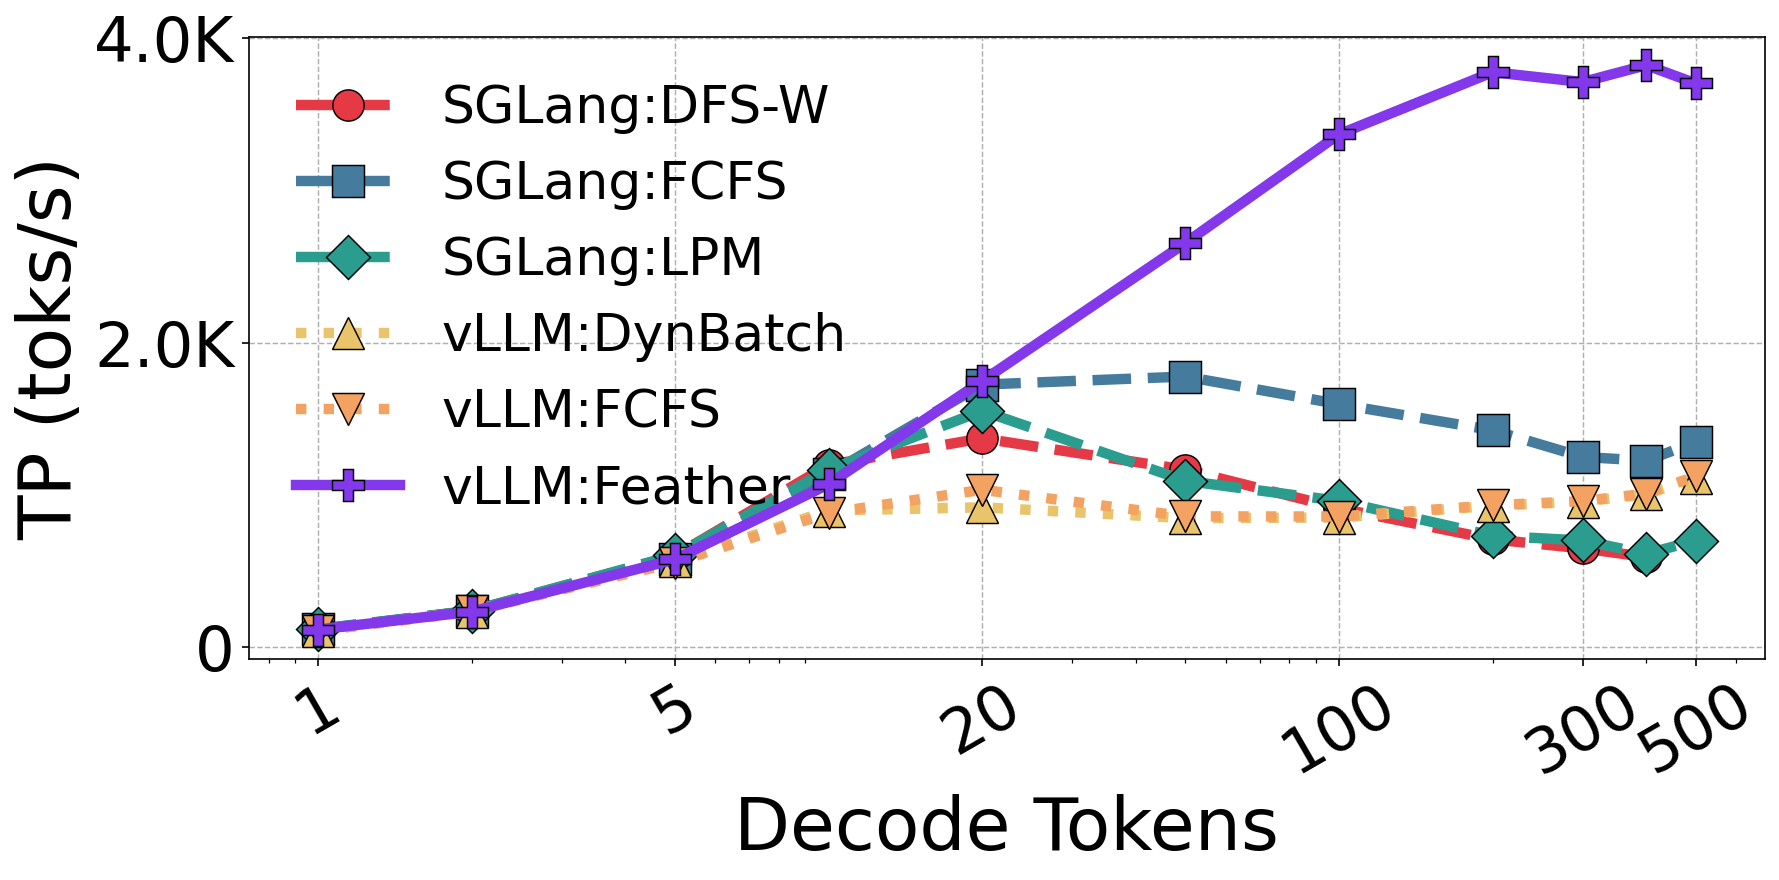
\includegraphics[width=\linewidth]{results/decode_tokens_plots/throughput_vs_tok.png}
    \caption{Throughput}
    \label{fig:tp_vs_tok_l_5000}
\end{subfigure}
\hfill
\begin{subfigure}{0.49\columnwidth}
    \centering
    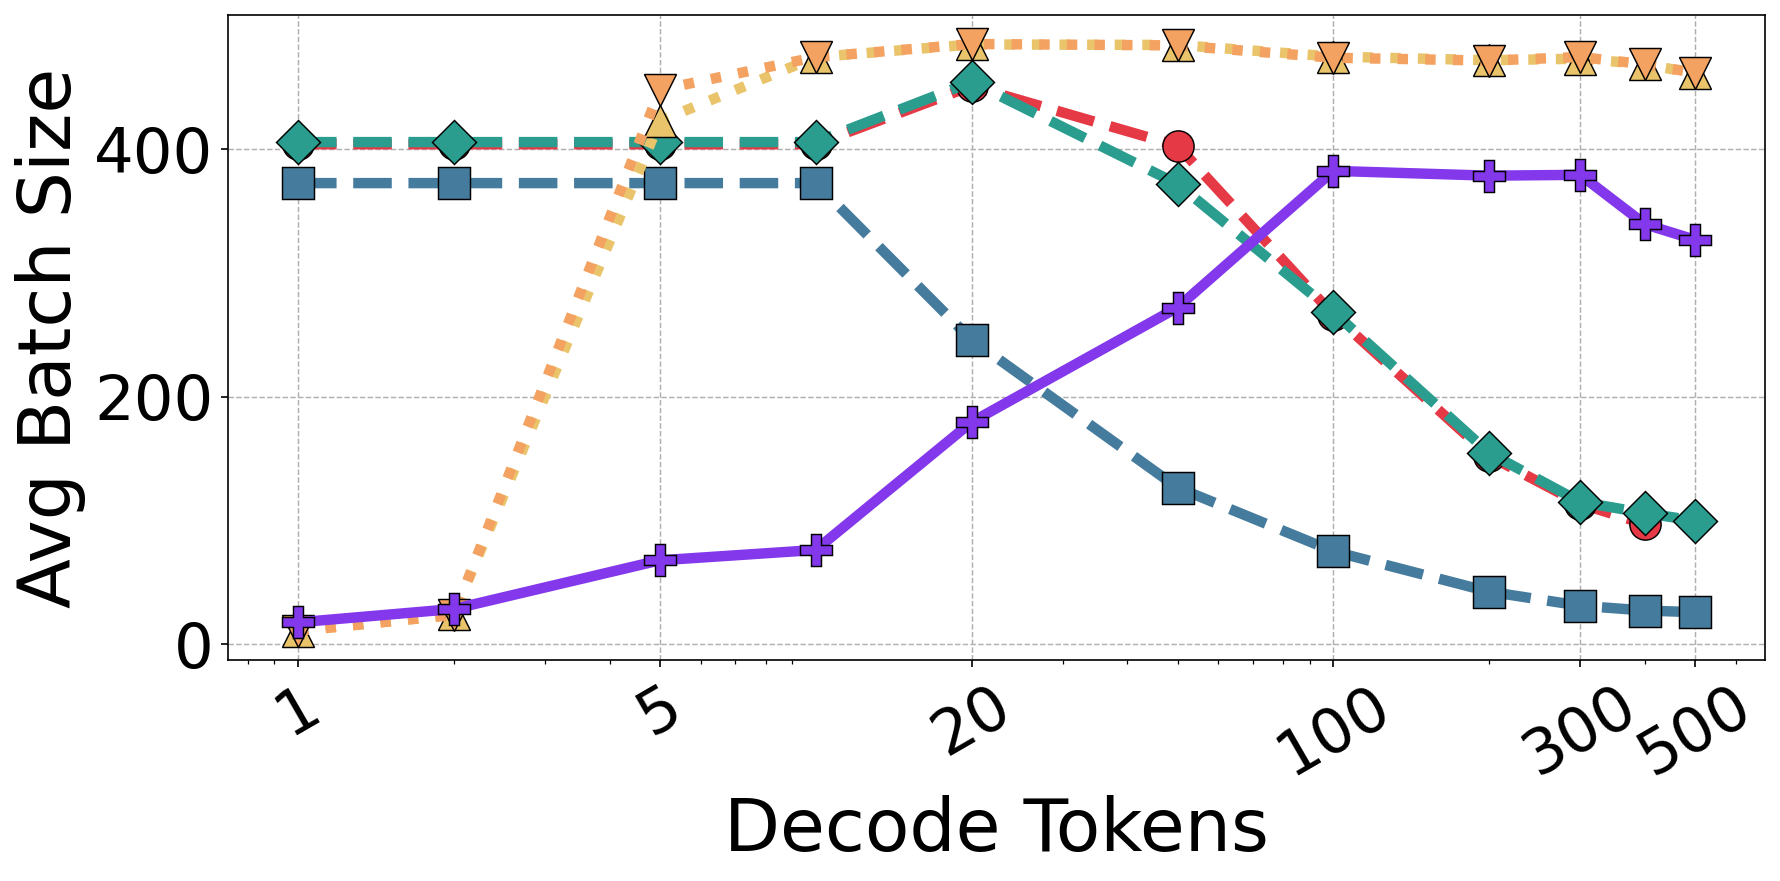
\includegraphics[width=\linewidth]{results/decode_tokens_plots/avg_batch_vs_tok.png}
    \caption{Average Batch Size}
    \label{fig:abs_vs_tok_l_5000}
\end{subfigure}
\caption{Varying Number of Decode Tokens}
\label{fig:num_decode_tokens}
\vspace{-15pt}
\end{figure}

\vspace{-5pt}

\subsubsection*{Varying Number of Decode Tokens}
Figures~\ref{fig:tp_vs_tok_l_5000} and \ref{fig:abs_vs_tok_l_5000} show throughput and average batch size as functions of decode tokens per request. Each decode requires a full sweep over the KV cache. The policies exhibit two regimes separated by a crossover around 20 decode tokens. In the prefill-dominated regime (1--20 tokens), all policies behave similarly: throughput increases modestly, and batch sizes converge as prefills limit the impact of locality-aware scheduling. Beyond 20 tokens, the policies diverge sharply. \Feather scales strongly with decode length, reaching $\sim$3800 toks/s at 200 tokens—over $3\times$ higher than SGLang policies. This gain arises from two factors. First, longer decode phases amplify locality across repeated KV cache sweeps. Second, a greater number of decode iterations allows the scheduler to accumulate more same-prefix requests, forming larger, more homogeneous batches. Together, these effects drive the steady increase in \Feather's batch size and throughput. SGLang policies follow the opposite trajectory in batch size. Because shared prefix tokens count toward the token budget, each prefill consumes $\sim$5K tokens, while each decode step contributes only one token. As the decode length increases, fewer prefills occur per step, reducing the number of new requests for batching.

\vspace{-5pt}

\subsubsection*{Varying Number of Shared Prefix Tokens}
Figure~\ref{fig:tp_vs_sys_eval} shows throughput across the length of the shared prefix. As expected, longer prefixes increase prefill compute and KV cache pressure, reducing throughput across policies. \Feather's advantage grows with prefix length, driven by higher locality gains as sequences lengthen.

\begin{figure}[t]
\centering
\begin{minipage}{0.49\columnwidth}
    \centering
    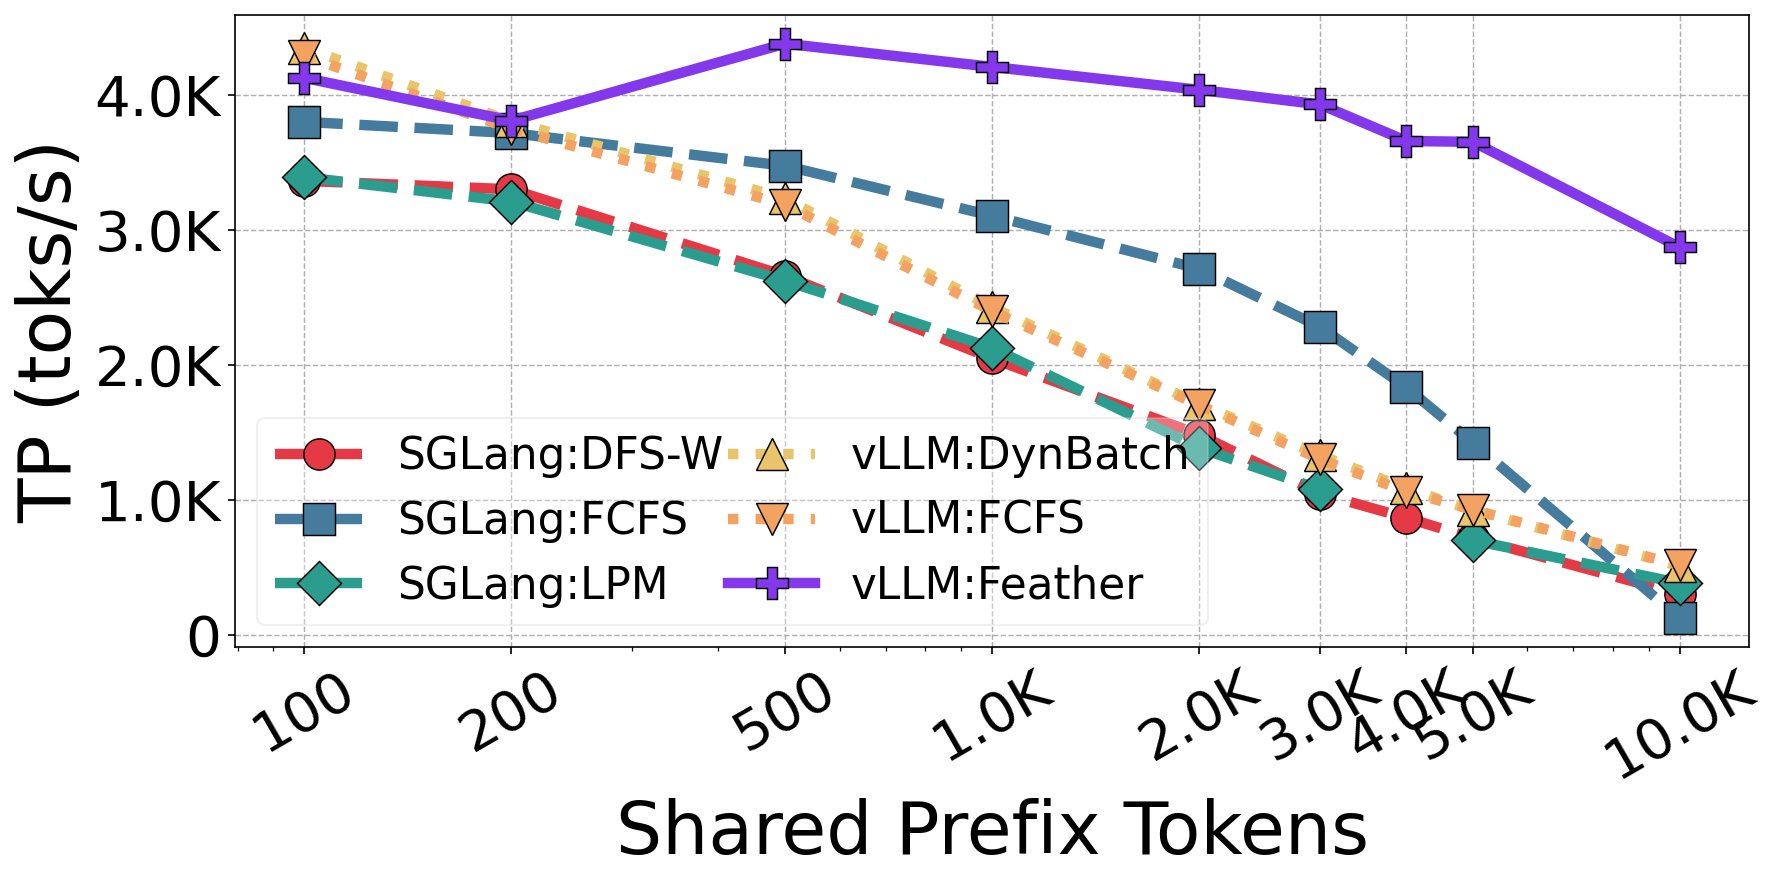
\includegraphics[width=\linewidth]{results/sys_prompt_tokens_plots/throughput_vs_sys_prompt_tokens.png}
    \caption{Varying Shared Prefix Tokens}
    \label{fig:tp_vs_sys_eval}
\end{minipage}
\hfill
\begin{minipage}{0.49\columnwidth}
    \centering
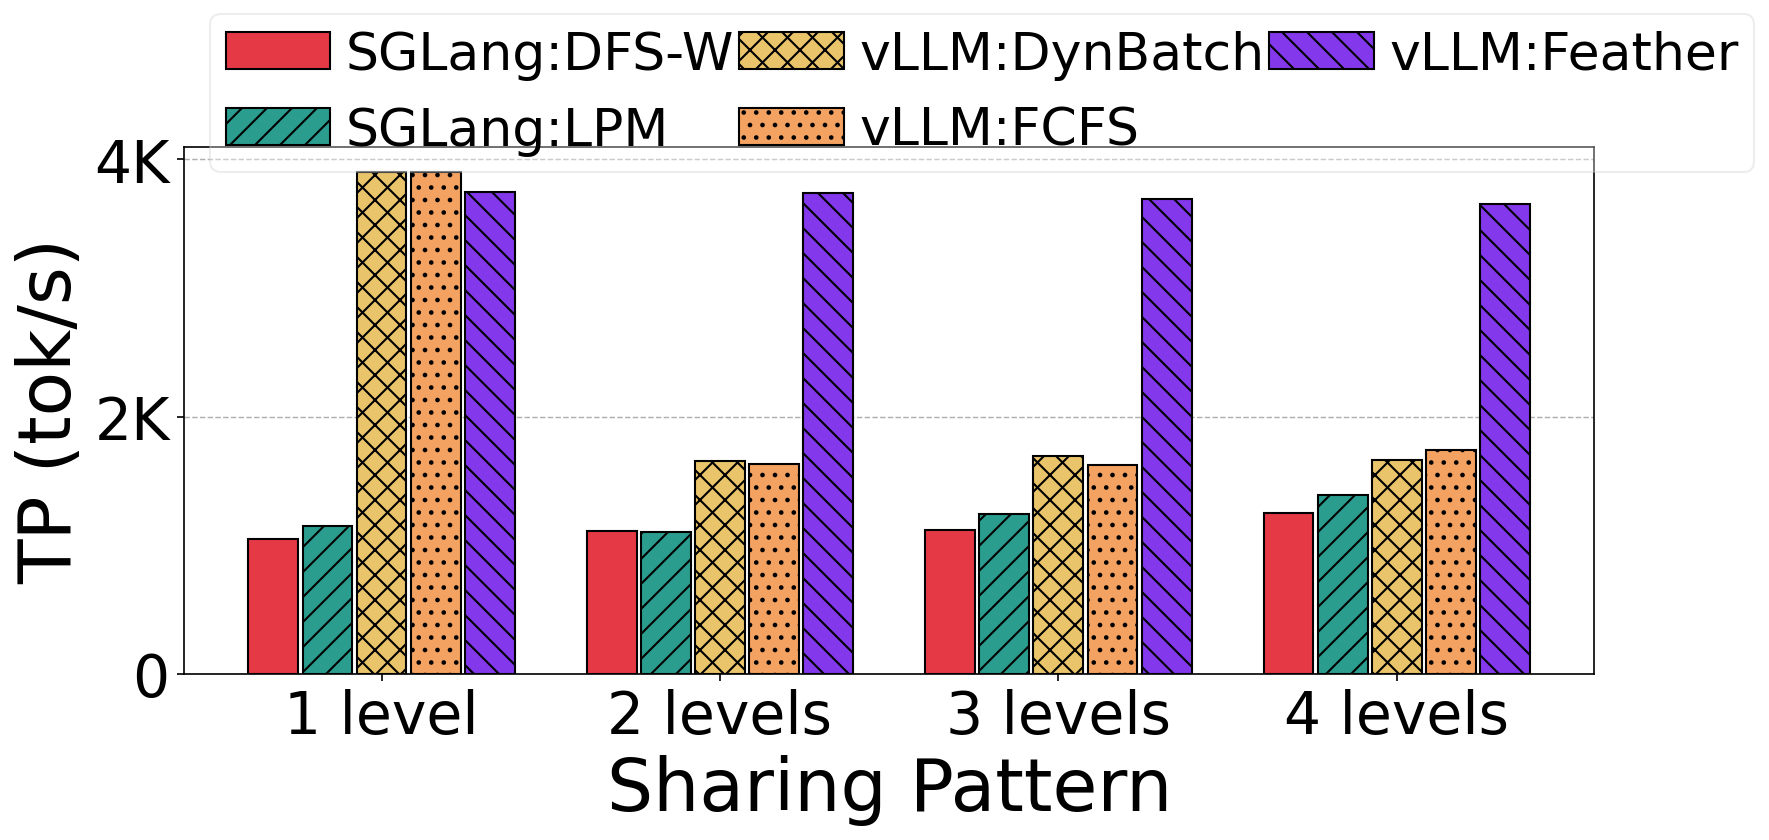
\includegraphics[width=\linewidth]{results/radix_tree_mode_barcharts/sys1000/throughput_by_mode.png}
\caption{Varying Radix Tree Sharing Levels}
\label{fig:tp_vs_rad_eval}
\end{minipage}
\vspace{-20pt}
\end{figure}

\vspace{-5pt}

\subsubsection*{Varying Models}
\Feather consistently achieves the highest throughput across models and outperforms baselines in nearly all cases. Its relative throughput advantage increases with model size, as larger models spend more time in attention, amplifying the benefits of KV-cache locality exploited by \Feather. All graphs are shown in \S\ref{subsec:across_models}. We also compare \Feather with other policies (\S\ref{subsec:results_across_longchat_model}) for the LongChat 13B model, where we achieve up to 22$\times$ higher throughput compared to vLLM's FCFS for larger number of prefix groups.

\begin{figure}[t]
\centering
\begin{minipage}{0.49\columnwidth}
   \centering

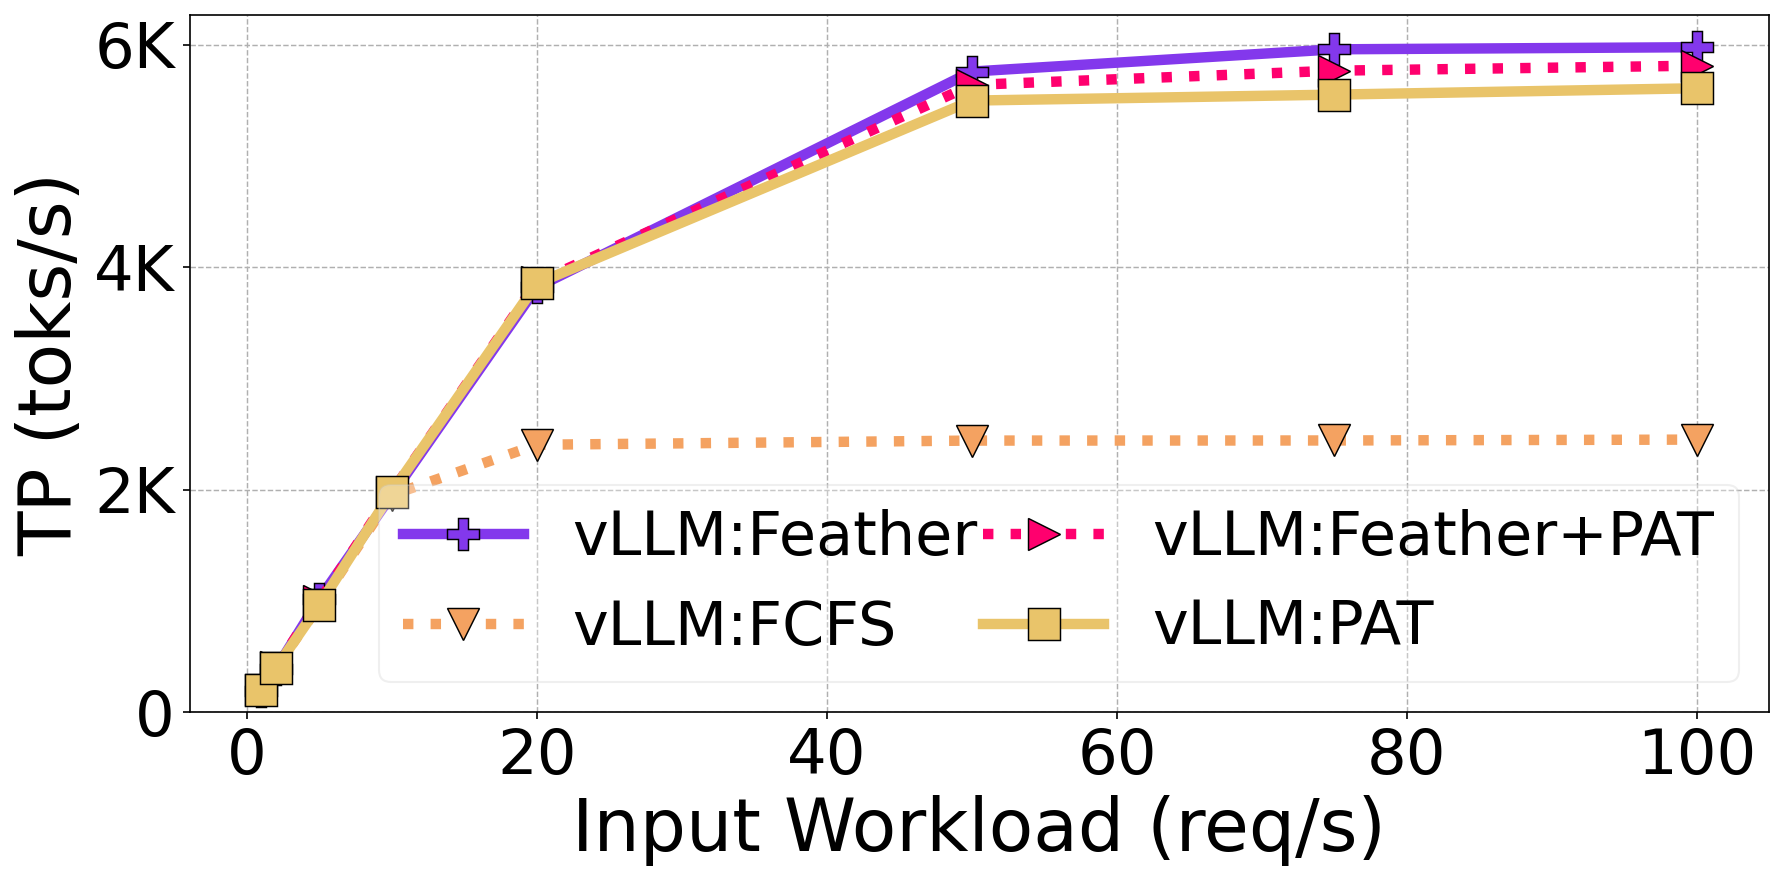
\includegraphics[width=\linewidth]{results/req_per_sec_plots/throughput_vs_rps_pat_fcfs_feather.png}
\caption{\Feather vs PAT}
\label{fig:throughput_vs_rps_pat_fcfs_feather_eval}
\end{minipage}
\hfill
\begin{minipage}{0.49\columnwidth}
   \centering
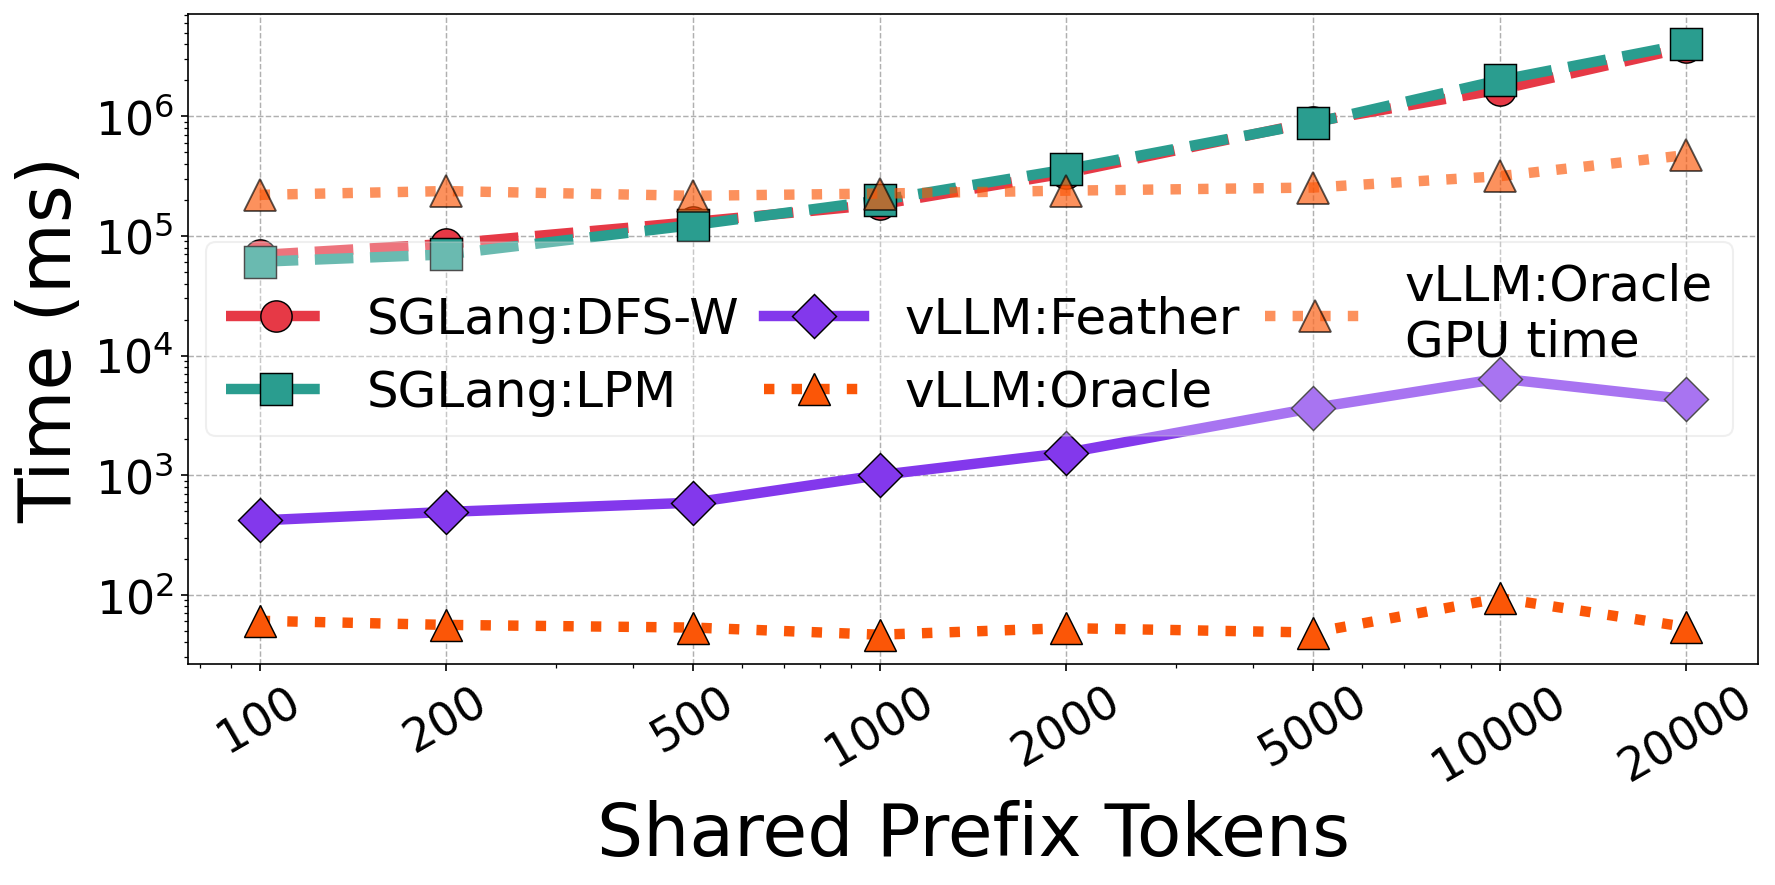
\includegraphics[width=\linewidth]{results/profile_sum_vs_sys_prompt_tokens.png}
\caption{CPU overhead}
\label{fig:profile_sum_vs_sys_prompt_tokens_eval}
\end{minipage}
\vspace{-20pt}
\end{figure}

\vspace{-5pt}

\subsubsection*{Varying Radix Tree Levels}
Figure~\ref{fig:tp_vs_rad_eval} shows throughput under different radix-tree sharing levels (seen in \S\ref{subsec:significance_of_prefix_homogeneity}). All experiments use a fixed total sequence length of 4000 tokens per request. For baseline policies like vLLM's FCFS, going from 1 to 2 or more levels of the radix tree reduces the locality in KV cache traversal and, hence, degrades throughput. In contrast, \Feather actively preserves prefix homogeneity within batches, leading to stable throughput at all levels.

\vspace{-5pt}

\subsubsection*{Comparison with PAT}
Figure~\ref{fig:throughput_vs_rps_pat_fcfs_feather_eval} compares throughput across varying request rates for PAT, vLLM (FCFS), and \Feather on an A100-80GB GPU. PAT is specifically optimized for this hardware through custom prefix-aware kernels. Despite this, \Feather consistently matches or outperforms PAT across all request rates, demonstrating strong performance even on different hardware. This is particularly notable because \Feather operates purely at the scheduling layer, without any kernel-level modifications. A naive integration of \Feather and PAT performs quite similarly to \Feather over most regimes. As future work, we aim to more tightly integrate \Feather with prefix-aware attention kernels, enabling deeper co-design between the scheduler and kernel-level optimizations to further improve performance.

\vspace{-5pt}

\subsection{Micro-Benchmarks}
\subsubsection*{Comparing Scheduler Compute Overhead across Different Policies}
Figure~\ref{fig:profile_sum_vs_sys_prompt_tokens_eval} shows the CPU scheduling overhead for each policy across different shared prefix lengths. We include an Oracle policy where the caller supplies prefix group identifiers with each request. This allows the scheduler to batch same-prefix requests without any prefix matching overhead, resulting in effectively zero scheduling cost while preserving locality. We also show the GPU execution time for this Oracle scheduling policy. All three realistic policies—\Feather, LPM, and DFS-W— incur higher overhead as the prefix length increases due to deeper radix-tree traversals and larger key comparisons. However, their growth rates diverge significantly. At 20K tokens, LPM and DFS-W incur roughly 1,000$\times$ higher overhead than \Feather. At larger sequence lengths, their scheduling overhead exceeds the Oracle GPU execution time by up to 10$\times$. This indicates that CPU overhead alone can negate the benefits of cache-aware batching. In contrast, \Feather remains below 1\% of GPU execution time across the entire range. We do a detailed analysis of the overheads of LPM and DFS-W policies in \S\ref{subsec:scheduling-complexity}.

\vspace{-5pt}

\begin{figure}[t]
\captionsetup[subfigure]{labelformat=simple}
    \renewcommand\thesubfigure{(\alph{subfigure})}
\centering
\begin{subfigure}{0.49\columnwidth}
    \centering
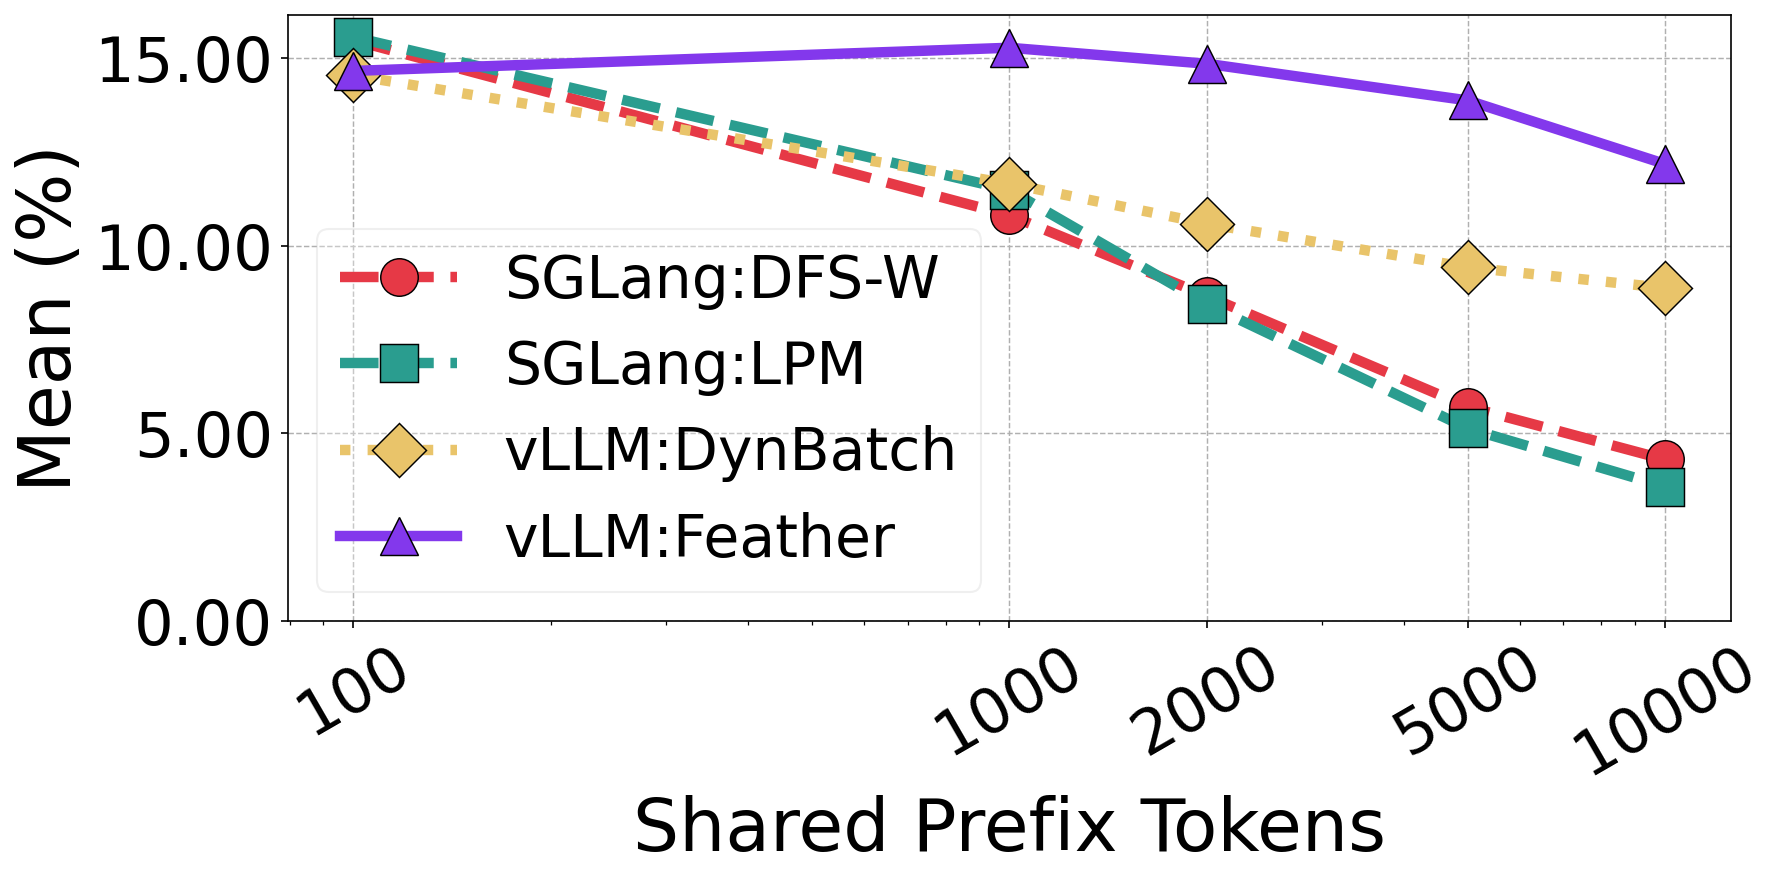
\includegraphics[width=\linewidth]{results/sys_prompt_tokens_plots/mean_dram_vs_sys_prompt_tokens.png}
\caption{Mean}
\label{fig:mean_drama_vs_sys_prompt_tokens}
\end{subfigure}
\hfill
\begin{subfigure}{0.49\columnwidth}
   \centering
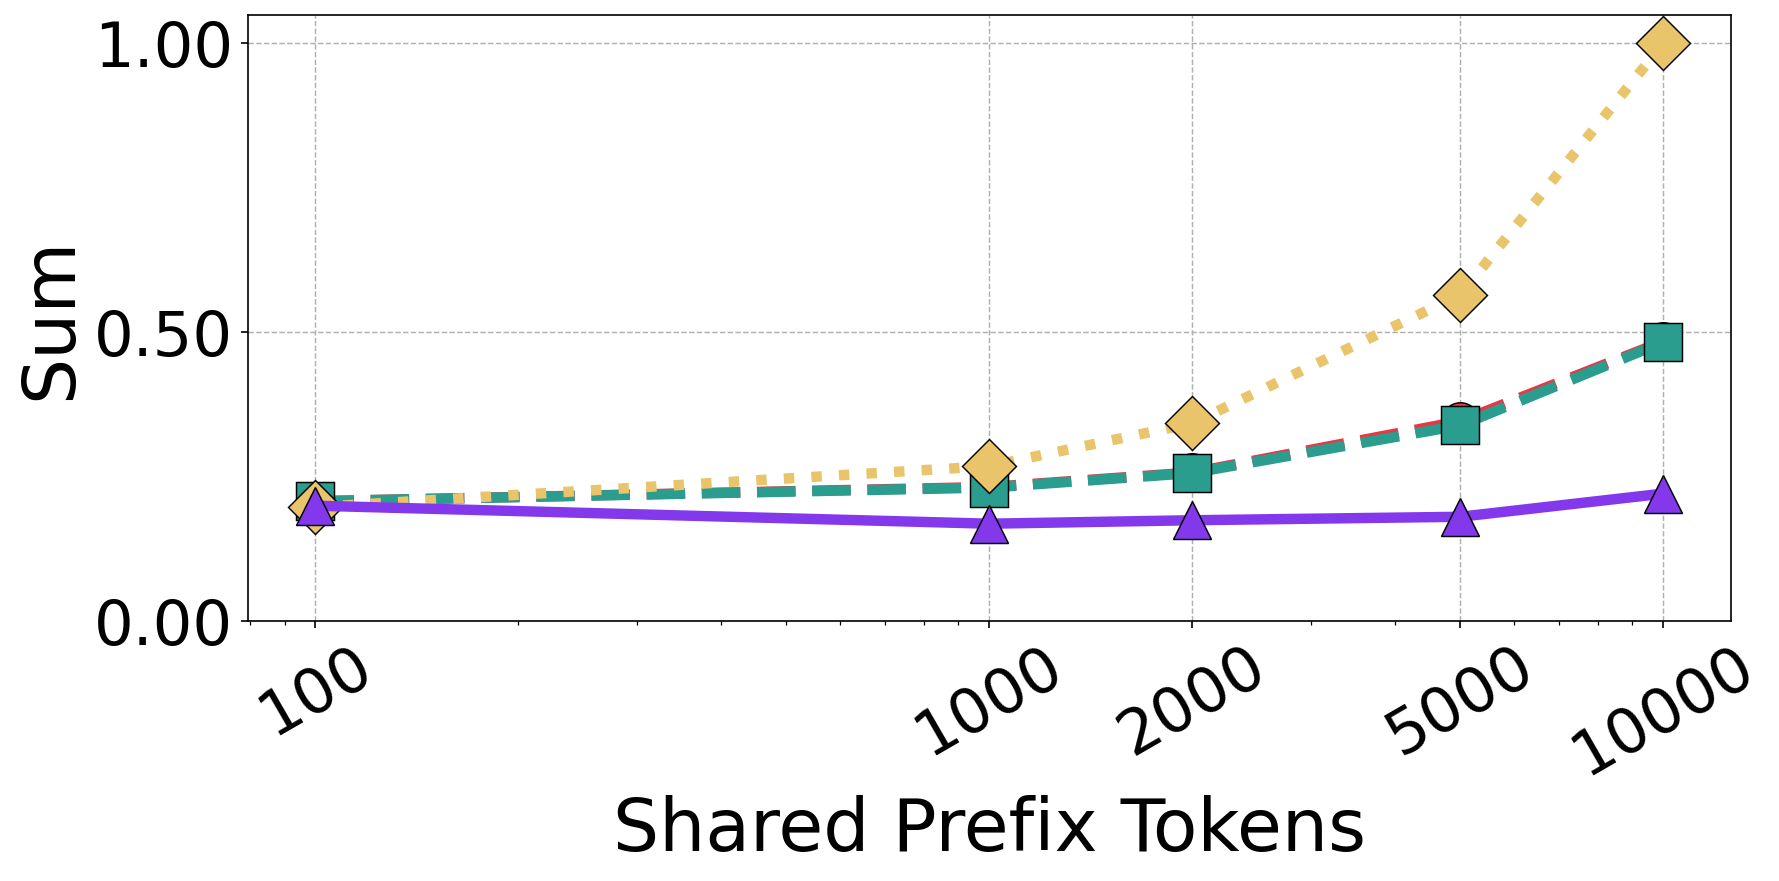
\includegraphics[width=\linewidth]{results/sys_prompt_tokens_plots/sum_dram_vs_sys_prompt_tokens.png}
\caption{Sum}
\label{fig:sum_dram_vs_sys_prompt_tokens}
\end{subfigure}
\caption{DRAM Bandwidth Utilization}
\label{fig:microbenchmark}
\vspace{-15pt}
\end{figure}

\begin{figure}[t]
\captionsetup[subfigure]{labelformat=simple}
    \renewcommand\thesubfigure{(\alph{subfigure})}
\centering
\begin{subfigure}{0.49\columnwidth}
    \centering
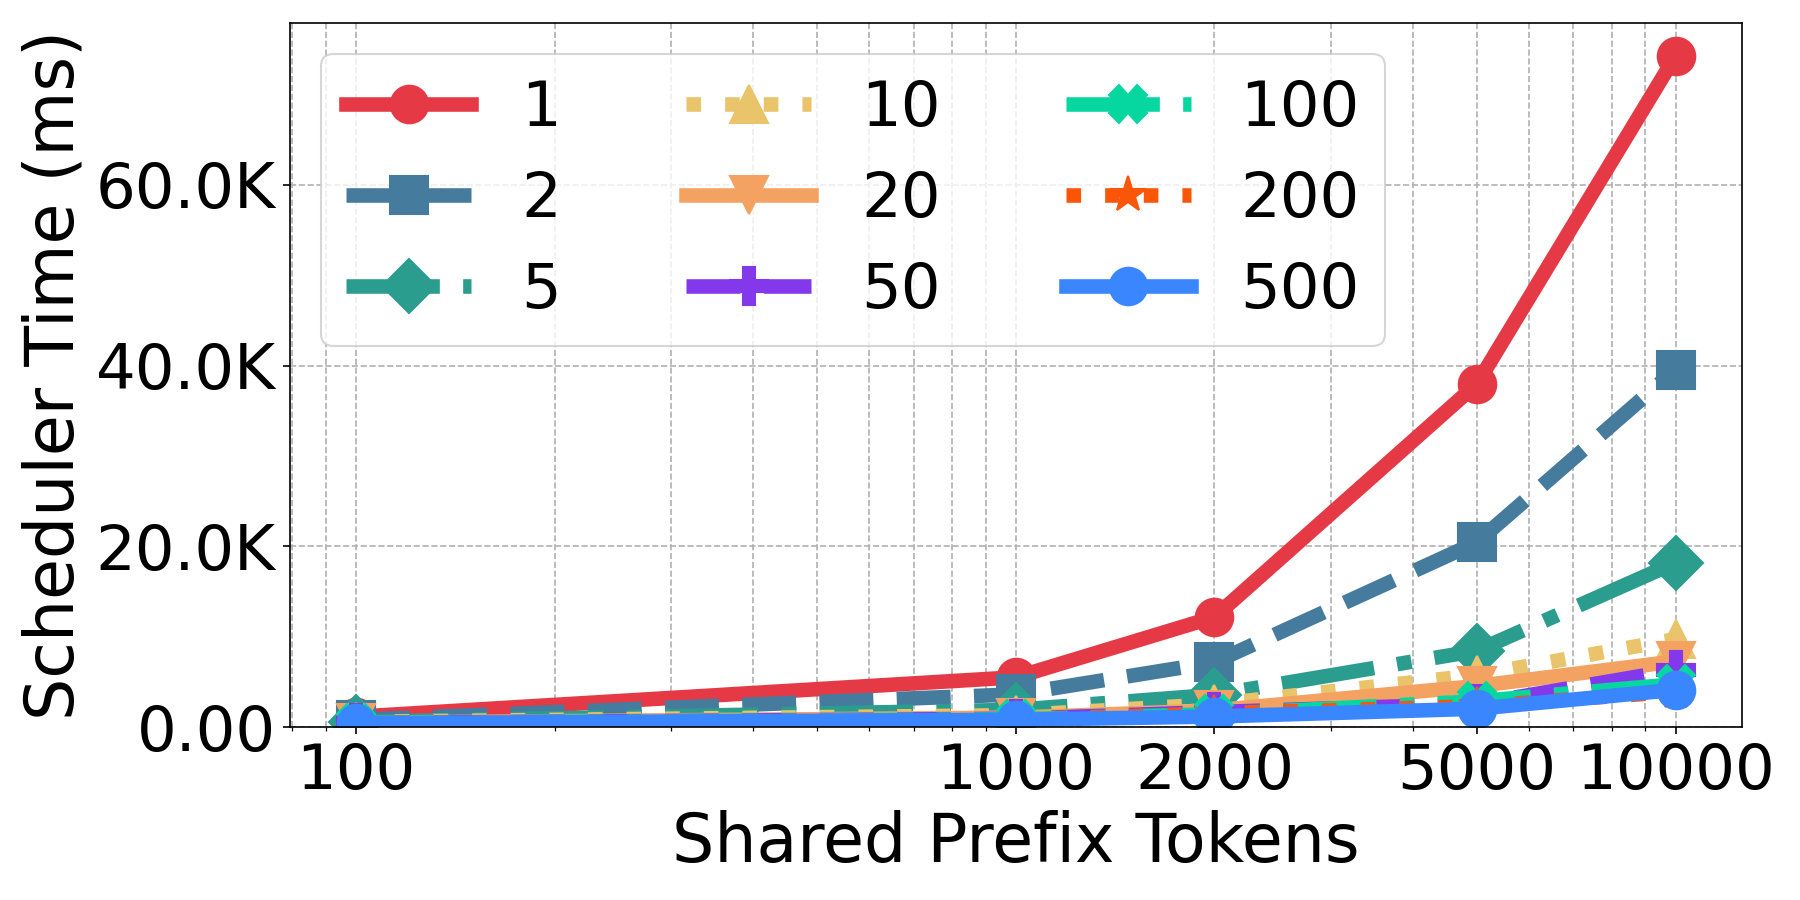
\includegraphics[width=\linewidth]{results/functotals_vs_systok_chunks.png}
\caption{CPU Scheduler Overhead}
\label{fig:functotals_vs_systok_chunks}
\end{subfigure}
\hfill
\begin{subfigure}{0.49\columnwidth}
    \centering
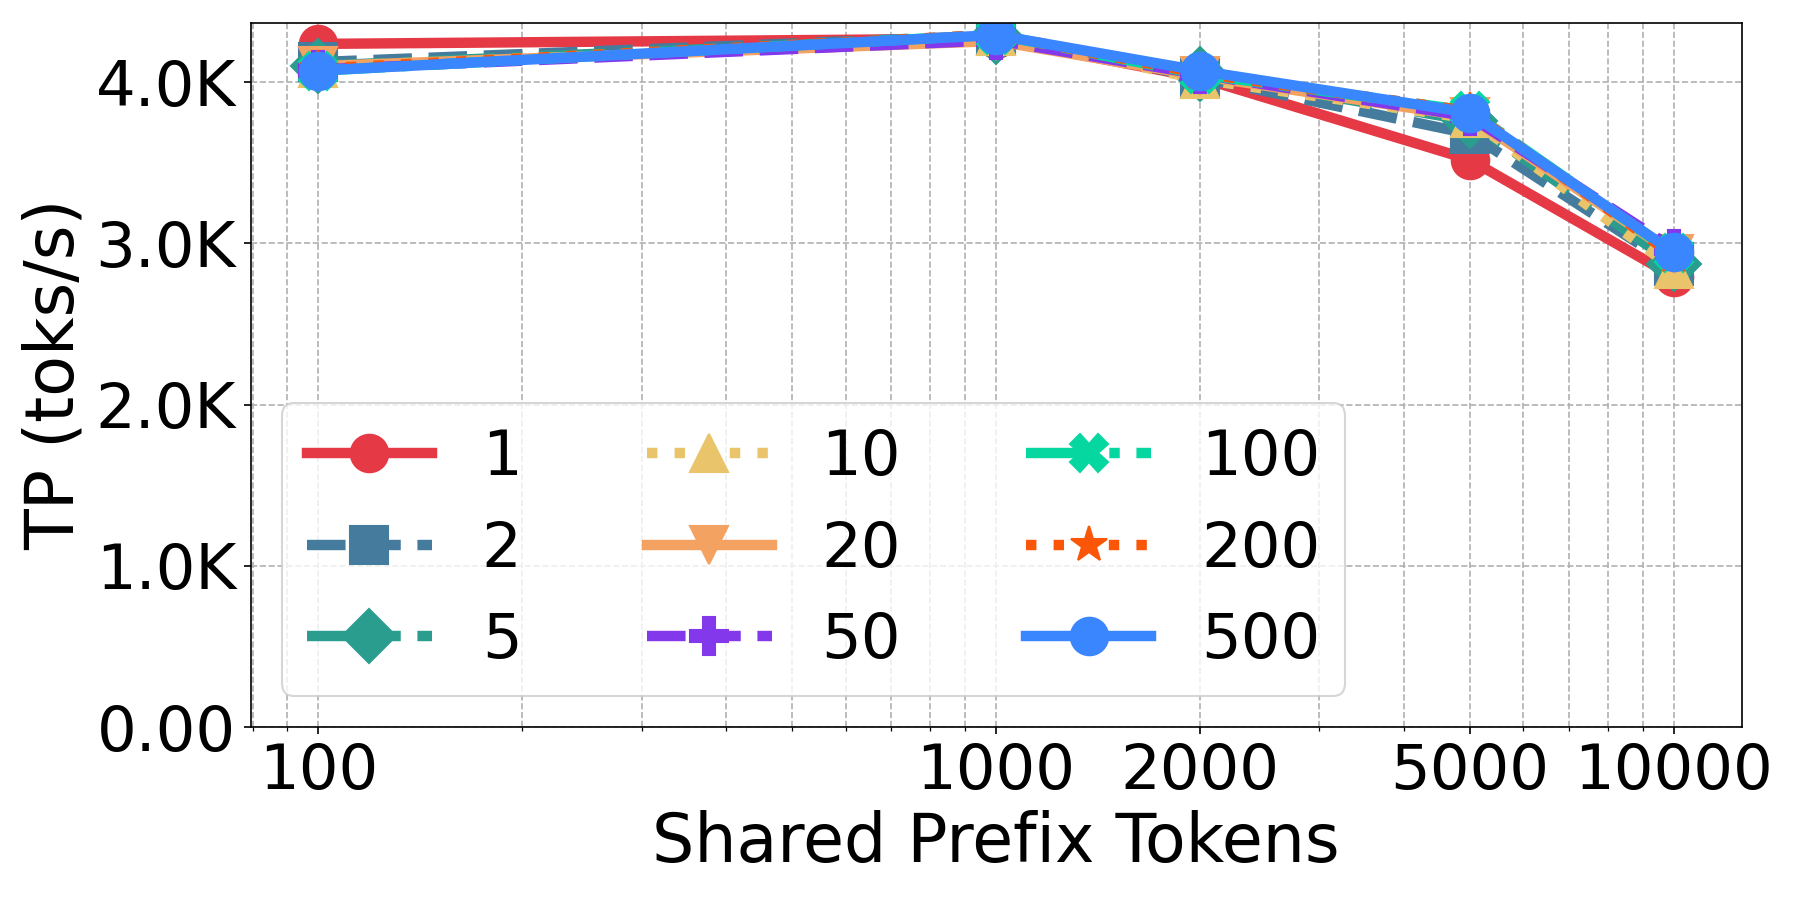
\includegraphics[width=\linewidth]{results/throughput_vs_systok_chunks.png}
\caption{Throughput}
\label{fig:throughput_vs_systok_chunks}
\end{subfigure}
\caption{Sensitivity to Chunk Size}
\label{fig:chunk_size_sensitivity}
\vspace{-18pt}
\end{figure}

\subsubsection*{Mean DRAM Activity across Various Sequence Lengths}
Figure~\ref{fig:mean_drama_vs_sys_prompt_tokens} shows mean DRAM bandwidth utilization, while Figure~\ref{fig:sum_dram_vs_sys_prompt_tokens} shows the total DRAM usage over the full inference duration (a proxy for total memory accessed) across policies and shared prefix lengths. \Feather consistently achieves the highest bandwidth utilization due to improved spatial locality, leading to more effective prefetching. Furthermore, more homogeneous batches also increase temporal locality, which is reflected in lower total DRAM usage. SGLang's DFS-W and LPM exhibit lower mean DRAM utilization because of CPU scheduler stalls. However, they also achieve lower normalized total DRAM usage, as their prefix-aware scheduling occasionally forms homogeneous batches, allowing them to partially benefit from memory locality.

\vspace{-5pt}

\subsubsection*{Effect of Chunk Size}
Figures~\ref{fig:functotals_vs_systok_chunks} and~\ref{fig:throughput_vs_systok_chunks} show CPU overhead and throughput across shared prefix lengths for different chunk sizes in \Feather's CHT. Increasing the chunk size reduces CPU overhead by enabling coarser-grained matching; a chunk size of 1 is equivalent to an exact radix tree. Overhead rises with prefix length due to more hash comparisons, while throughput declines due to higher KV cache memory pressure. At larger prefix lengths, the overhead gap between chunk size 1 and larger sizes widens substantially, yet throughput remains similar across all chunk sizes, suggesting that the CPU scheduling cost, even at the finest granularity, is not the primary bottleneck in our CHT. Overall, CHT is robust against chunk size selection, and even its radix tree-equivalent configuration (chunk size 1) achieves significantly better efficiency than a conventional radix tree.

\vspace{-5pt}

\subsection{Ablation Study}
\subsubsection*{What if we Replace the Chunked Hash Tree with a Radix Tree?}
Figure~\ref{fig:throughput_vs_sys_prompt_tokens_bar} compares throughput and TBT when replacing CHT with a radix tree under the same RL policy. Across all prefix lengths, the radix tree yields much lower throughput. Despite homogeneous RL batching, higher CPU overhead causes frequent GPU stalls. This appears as higher TBT, indicating GPU idle time due to scheduling delays. CHT avoids this by reducing scheduling overhead, enabling higher GPU utilization and throughput.

\begin{figure}[t]
\centering
\begin{minipage}{0.49\columnwidth}
   \centering
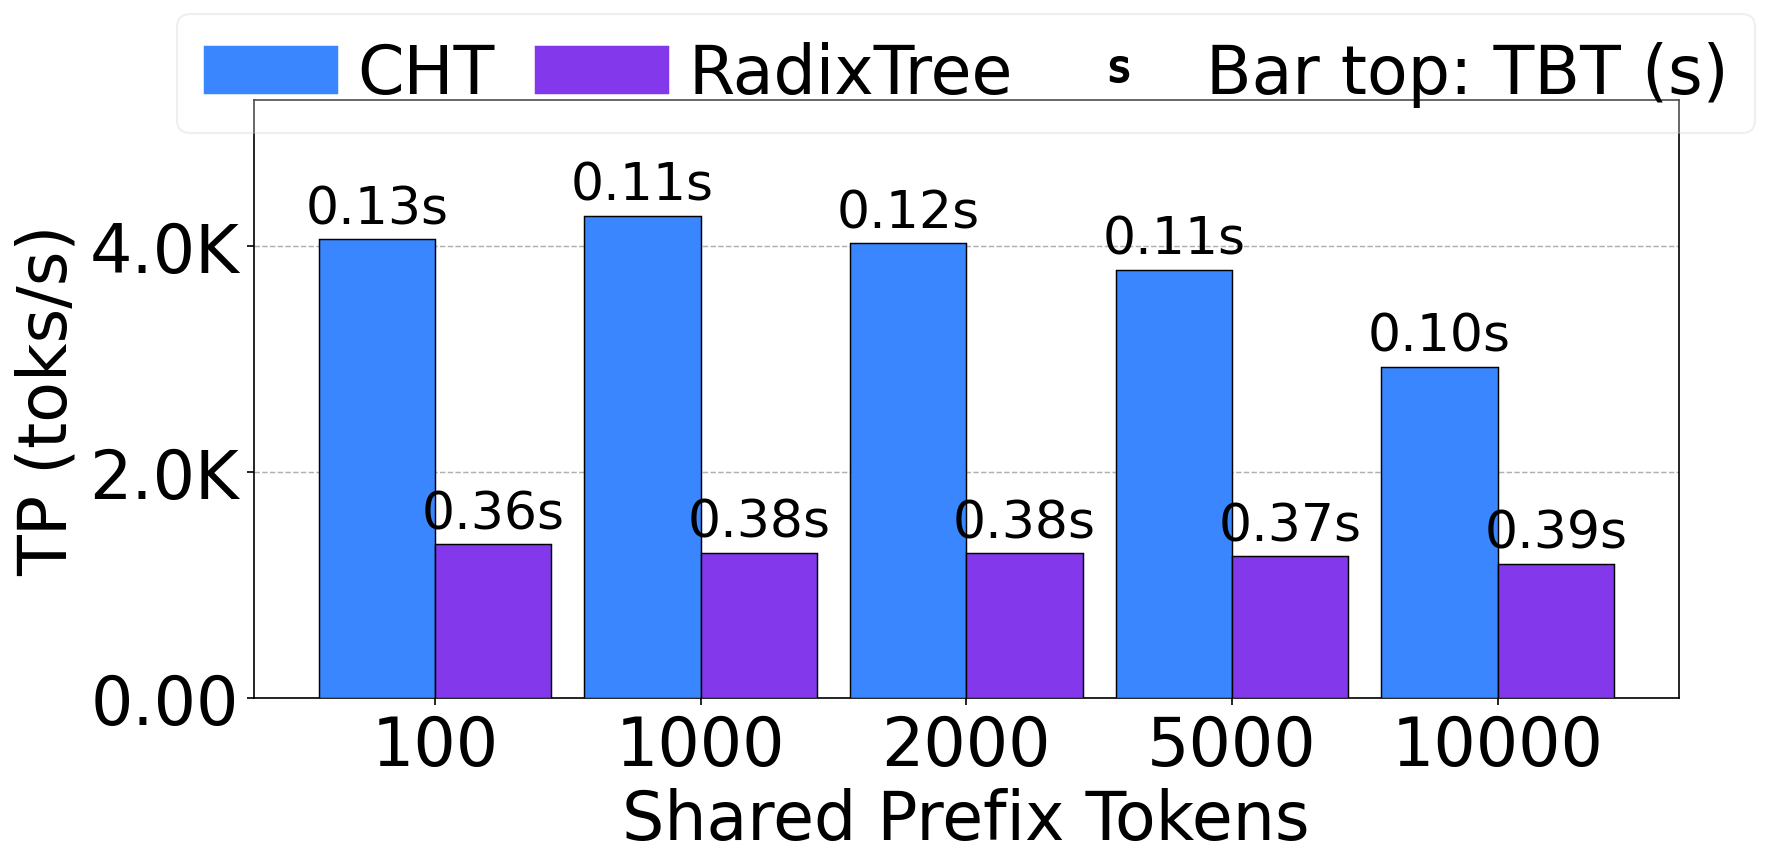
\includegraphics[width=\linewidth]{results/sys_prompt_tokens_plots_ablation/throughput_vs_sys_prompt_tokens_bar.png}
\caption{CHT vs. Radix Tree}
\label{fig:throughput_vs_sys_prompt_tokens_bar}
\end{minipage}
\hfill
\begin{minipage}{0.49\columnwidth}
   \centering
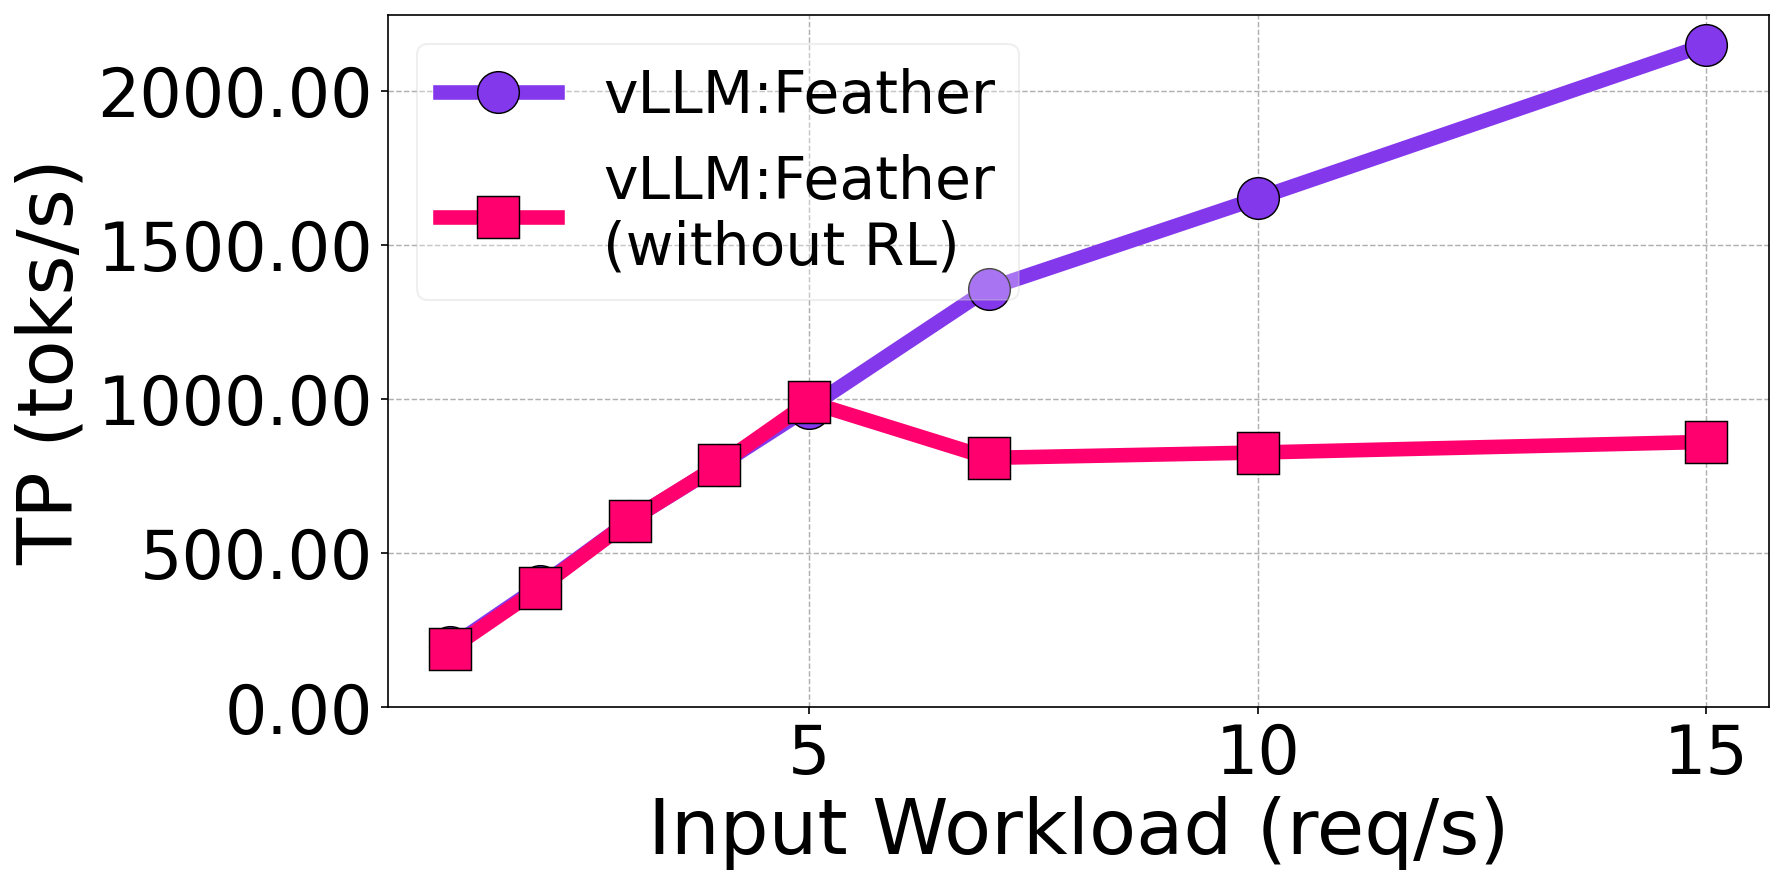
\includegraphics[width=\linewidth]{results/req_per_sec_plots_ablation/throughput_vs_rps.png}
\caption{\Feather: with and without RL}
\label{fig:tp_vs_req_per_sec_ablation}
\end{minipage}
\vspace{-25pt}
\end{figure}

\vspace{-5pt}

\subsubsection*{What if We Remove RL?}
Figure~\ref{fig:tp_vs_req_per_sec_ablation} compares throughput with and without RL at low input rates. Without RL, CHT still selects the best request, but batching never halts and always maximizes batch size. At <5 req/s, removing RL has little effect. Both fall back to FCFS, adding requests to keep GPUs utilized. Beyond this, the behaviors diverge. With RL, \Feather detects homogeneous requests and stops batching at the right time, achieving higher throughput despite smaller average batch sizes. At higher rates than shown in the figure, large pools enable even non-RL to form ${\sim}500$-request homogeneous batches, leading the two curves to converge. These results show that \Feather's RL policy makes load-aware decisions: it falls back to FCFS under low utilization to avoid GPU starvation, and closes batch formation when homogeneity is achievable, maximizing overall throughput.

Interested readers can see \S\ref{sec:additional_results_of_feather} for additional results.